% The knowledge graph's main classes (run5_build_outputs.MAIN_CLASSES; their subclasses in the papers' class table): entities as hubs (blue), source
% rows (orange), the storm x country rows built here (green).
% Compile: pdflatex fig_kg.tex, cropped by statistics/figure_kg.py -> included by both journal builds.
% Drawn at the figures' common width (13.3 cm) in Helvetica at 8 pt, as the other figures (Arial, 8 pt), so all print at one size.
\documentclass[10pt]{article}
\usepackage[paperwidth=30cm,paperheight=30cm,margin=1cm]{geometry}
\usepackage[T1]{fontenc}
\usepackage{helvet}
\renewcommand{\familydefault}{\sfdefault}
\usepackage{graphicx}
\usepackage{tikz}
\usepackage{hyperref}
\pagestyle{empty}
\usetikzlibrary{arrows.meta,positioning,fit,backgrounds}
% Colour-blind-safe palette (blue, orange, aqua), light fills under dark text
\definecolor{thing}{HTML}{DCEAFB}
\definecolor{edge}{HTML}{2A78D6}
\definecolor{srcfill}{HTML}{FCE3D7}
\definecolor{srcedge}{HTML}{EB6834}
\definecolor{recfill}{HTML}{D5F2E7}
\definecolor{recedge}{HTML}{1BAF7A}
\definecolor{ink}{HTML}{0B0B0B}
\definecolor{muted}{HTML}{52514E}
\definecolor{ext}{HTML}{EEF0F3}
\begin{document}
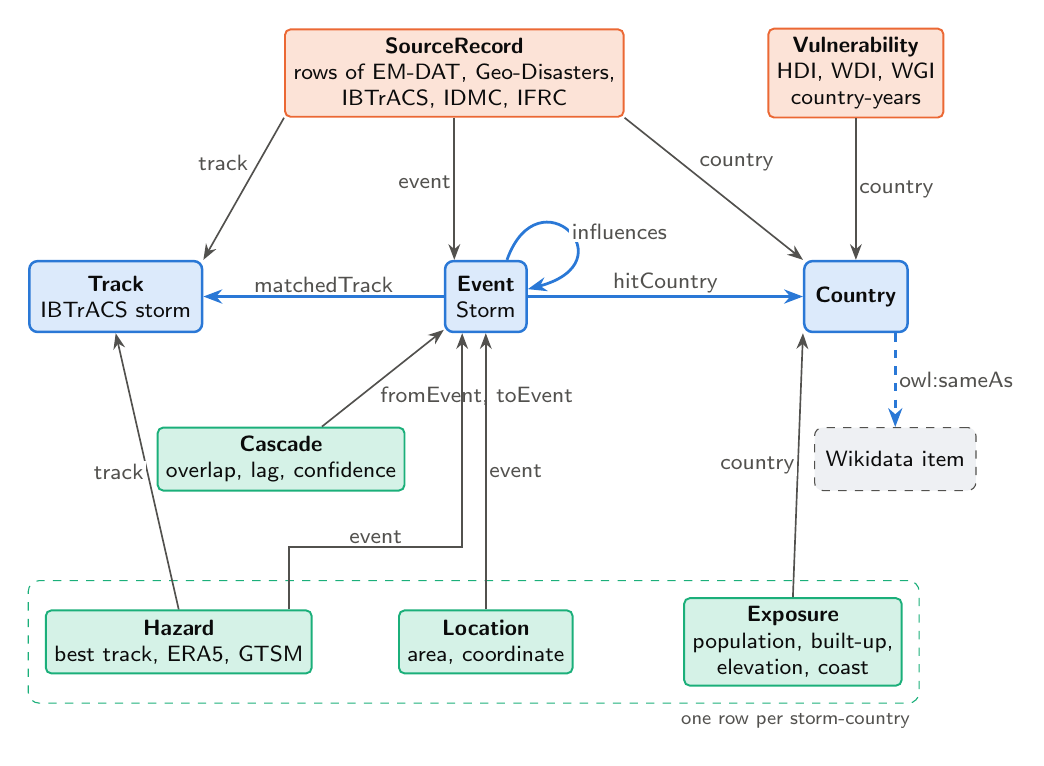
\begin{tikzpicture}[font=\footnotesize, text=ink, y=0.86cm,
  thing/.style={draw=edge, fill=thing, rounded corners=3pt, line width=0.9pt, align=center, inner sep=4pt, minimum height=9mm},
  src/.style={draw=srcedge, fill=srcfill, rounded corners=2pt, line width=0.7pt, align=center, inner sep=3pt, minimum height=8mm},
  rec/.style={draw=recedge, fill=recfill, rounded corners=2pt, line width=0.7pt, align=center, inner sep=3pt, minimum height=8mm},
  ext/.style={draw=muted, fill=ext, dashed, rounded corners=3pt, align=center, inner sep=4pt, minimum height=8mm},
  rel/.style={-{Stealth[length=2.4mm]}, line width=1pt, draw=edge},
  key/.style={-{Stealth[length=2mm]}, line width=0.6pt, draw=muted},
  lab/.style={font=\footnotesize, text=muted, fill=white, inner sep=1pt},
  sub/.style={font=\scriptsize, text=muted}]

% entities (blue): the hubs the rows point at
\node[thing] (event) at (0,1.5) {\textbf{Event}\\Storm};
\node[thing] (country) at (4.7,1.5) {\textbf{Country}};
\node[thing] (track) at (-4.7,1.5) {\textbf{Track}\\IBTrACS storm};
\node[ext] (wd) at (5.2,-0.9) {Wikidata item};

% relations between entities
\draw[rel] (event) -- node[lab, above] {hitCountry} (country);
\draw[rel] (event) -- node[lab, above] {matchedTrack} (track);
\draw[rel] (event.60) .. controls +(0.4,1.3) and +(1.3,0.4) .. node[lab, right] {influences} (event.10);
\draw[rel, dashed] (country.south -| wd) -- node[lab, right] {owl:sameAs} (wd);

% source rows (orange)
\node[src] (srcrec) at (-0.4,4.8) {\textbf{SourceRecord}\\rows of EM-DAT, Geo-Disasters,\\IBTrACS, IDMC, IFRC};
\node[src] (vul) at (4.7,4.8) {\textbf{Vulnerability}\\HDI, WDI, WGI\\country-years};
\draw[key] (srcrec.south west) -- node[lab, pos=0.4, above left] {track} (track.north east);
\draw[key] (srcrec.south) -- node[lab, pos=0.45, left] {event} (srcrec.south |- event.north);
\draw[key] (srcrec.south east) -- node[lab, pos=0.4, above right] {country} (country.north west);
\draw[key] (vul) -- node[lab, right] {country} (country);

% rows built here (green)
\node[rec] (cas) at (-2.6,-0.9) {\textbf{Cascade}\\overlap, lag, confidence};
\draw[key] (cas) -- node[lab, pos=0.45, below right] {fromEvent, toEvent} (event);
\node[rec] (haz) at (-3.9,-3.6) {\textbf{Hazard}\\best track, ERA5, GTSM};
\node[rec] (loc) at (0,-3.6) {\textbf{Location}\\area, coordinate};
\node[rec] (exp) at (3.9,-3.6) {\textbf{Exposure}\\population, built-up,\\elevation, coast};
\begin{scope}[on background layer]
  \node[draw=recedge, dashed, rounded corners=4pt, inner sep=6pt, fit=(haz) (loc) (exp)] (sxc) {};
\end{scope}
\node[sub, anchor=north east] at (sxc.south east) {one row per storm-country};
\draw[key] (loc) -- node[lab, pos=0.5, right] {event} (event);
\draw[key] (exp.north) -- node[lab, pos=0.5, left] {country} (country.south west);
\draw[key] (haz.north) -- node[lab, pos=0.5, left] {track} (track.south);
\draw[key] ([xshift=-3mm]haz.north east) |- ([xshift=-3mm]event.south |- 0,-2.2) node[lab, pos=0.75, above] {event} -- ([xshift=-3mm]event.south);
\end{tikzpicture}
\end{document}
